%!TEX root = ../../Main.tex
\graphicspath{{Chapters/Indledning/}}
%-------------------------------------------------------------------------------

\chapter{Cross validation / Bootstrap}

When we are working with different machine learning models, we need two different data sets. The first set is often referred to as the training data set, and is used to create the model and define the curve seen in \ref{fig:logistic_regression}. The other dataset is referred to as the test set and is used to check if the model performs well. The data between the two sets can not be identical because we want to evaluate how the model performs on new data sets. 

Because we often dont have well defined test sets available, we need some methods to gain test data. Here we have several diffenret options. Some methods will not provide new data, but instead use the training data to estimate the test error (the performance). Another approach, which is the one discussed here, is a method where you hold out some part of the data, in the training process and use the hold out data as a test data set. 

When this is done with several different splits (different hold out sets) and we evaluate our model using the approach, we are achieving cross validation. The size of the hold our set can vary. If we choose the heaviest computational split, we only contains one sample in the hold out set. This is called leave-one-out-cross-validation LOOCV. 

\begin{figure}[H]
  \fbox{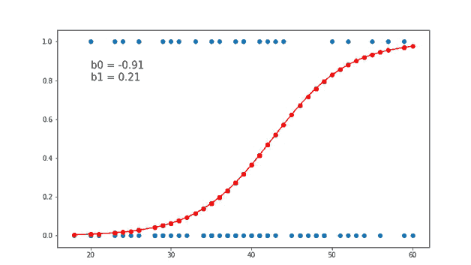
\includegraphics[width=230pt]{img/logistic_regression.PNG}}
  \centering
  \caption{Logistic regression model illustration}
  \label{fig:logistic_regression}
\end{figure}

When we have gained several different splits from using cross validation, we need to evaluate how our model performs in these different testing scenarios. We often use mean least square to evaluate our model. The formula for calculating this for our model with cross validation can be seen in \ref{eq:1}.

\begin{equation} \label{eq:1}
CV_{(k)} = \sum_{k=1}^{K} \frac{n_k}{n} MSE_k
\end{equation}

The need for cross validation comes from the fact that we easily can achieve overfitting if we 

